\subsection{Retry-Muster}

\textit{Retry} ist ein Architekturmuster, welches vorübergehende Fehler behandelt,
indem es fehlgeschlagene Operationen automatisch wiederholt, oft mit exponentiellen Backoff-Strategien.
Es eine bewährte Methode zur Verbesserung der Resilienz von Anwendungen,
die mit entfernten Diensten oder Netzressourcen kommunizieren~\cite{Meheden.2021}.
Wiederholungen sind ein entscheidender Aspekt für die Ausfallsicherheit von Anwendungen,
die in Containern oder in der Cloud ausgeführt werden~\cite{Haley.28.06.2018}.

\textit{Retry} ist eine effektive Technik zur Bewältigung vorübergehender Ausfälle in der
komponentenübergreifenden Kommunikation innerhalb eines Systems.
Azure und andere Cloud-Dienste und Client-SDKs bieten Wiederholungsfunktionalitäten, wie z.B.\ die Verwendung von
EnableRetryOnFailure von Entity Framework Core, um eine Wiederholungsstrategie für Datenbankaufrufe einzurichten~\cite{Haley.28.06.2018}.

% TODO Lesen: https://learn.microsoft.com/en-us/azure/architecture/patterns/retry

\paragraph{Bedingungen}

Für die Nutzung wird angenommen, dass die Fehlfunktion nur temporär ist.
Das Muster eignet sich besonders für Szenarien, in denen Fehler aufgrund von vorübergehender Nichtverfügbarkeit
oder Netzwerkkonnektivitätsproblemen auftreten~\cite{Meheden.2021}.

\begin{figure}[t]
    \centering
    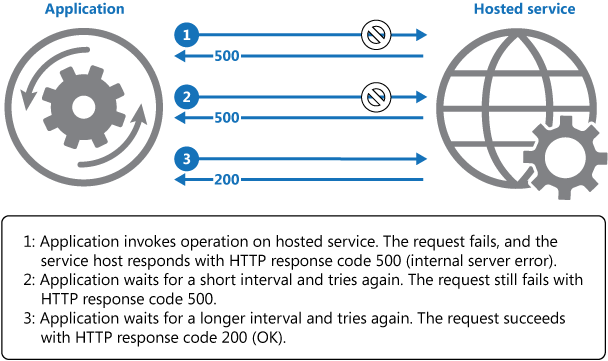
\includegraphics[width=\linewidth]{../images/retry-pattern}
    \caption{Aufrufen eines Vorgangs in einem gehosteten Dienst unter Verwendung von \textit{Retry}~\cite{Microsoft.}}
    \label{fig:retry}
    \Description{Kommunikationsvorgang zwischen einer Anwendung und einem gehosteten Service, zwei Aufrufe schlagen mit Status 500 fehl, der dritte ist erfolgreich (200).}
\end{figure}

Das Beispiel in Abbildung~\ref{fig:retry} zeigt, dass bei einem fehlerhaften Aufruf einer Dienstoperation
(z.B.\ Code 500) die Anwendung zunächst wartet und es erneut versucht.
Sollte der Fehler weiterhin bestehen, wird die Wartezeit verlängert, und schließlich
kann die Anfrage erfolgreich abgeschlossen werden (z.B.\ Code 200).

Die Wiederholungsstrategie muss jedoch an die spezifischen Geschäftsanforderungen angepasst werden.
So sollten weniger kritische Anfragen eher schnell scheitern, um die Benutzererfahrung nicht zu beeinträchtigen,
während bei größeren Verzögerungen die Anzahl der Wiederholungen begrenzt werden sollte.
Für erfolgreiche Implementierungen müssen Fehler gründlich protokolliert und getestet werden,
um potenzielle Probleme frühzeitig zu erkennen und zu beheben~\cite{Meheden.2021}.

Insgesamt trägt das Wiederholungsmuster dazu bei, die Fehlertoleranz und Stabilität von Anwendungen zu erhöhen,
indem es vorübergehende Fehler effektiv adressiert und die Auswirkungen auf die Geschäftsprozesse minimiert.

Die Kombination von Retry mit dem Circuit Breaker-Pattern kann die Ausfallsicherheit weiter erhöhen,
indem die Wiederholungsversuche nach einer bestimmten Anzahl von Fehlern gestoppt werden,
sodass das System sich erholen und anders reagieren kann, z.B.\ auf einen zwischengespeicherten Wert zurückgreifen kann.
% See ResilientHttpClient in https://azure.microsoft.com/de-de/blog/using-the-retry-pattern-to-make-your-cloud-application-more-resilient/

%\paragraph{Vorteile}

